\chapter{The Kakeya Problem in Finite Fields}
Before we can discuss the Kakeya problem in finite fields, and its rather surprising resolution, we ought to first discuss the origin and history of the problem. 
Work on the Kakeya problem can be traced back to the Russian mathematician Abram Besicovitch in 1917. While working on a problem in Riemann integration, Besicovitch reduced it to the question
of the existence of planar sets of measure zero which contain a line segment in every direction. In 1920, Besicovitch constructed such a set and published in a Russian Journal.

However, 1917 was a turbulent year as it marked the end of
the Russian Empire and the start of the Russian civil war. Due to this and the ensuing blockade of Russian ports there was scarce communication with the outside world.
Thus Besicovitch could not have known of a Japanese mathematician Kakeya who asked also in 1917 a related question: What is the smallest area of a convex set within which
one can rotate a needle by 180 degrees in the plane? Julius Pal answered this question in 1921 with the equilateral triangle. The 
more interesting problem without the convexity condition remained open. In 1924, after leaving the newly formed Soviet Union for Copenhagen, Besicovitch discovered this
problem and by modifying his previous construction produced a solution in 1925. This lead to the more general questions being asked about Kakeya sets in higher dimensions.
\begin{definition}[Kakeya Set in $\RR^n$]
    A Kakeya set is a set $A \subset \RR^n$ that contains a unit segment in every direction.
\end{definition}
Besicovitch's construction showed that these sets can have arbitrarily small measures, even attaining zero, in $\RR^2$. Further, a straightforward construction produces these measure zero sets in dimensions $> 2$.

The natural question then arises, what is the dimension of such sets? There are many notions of dimensions that can be investigated, but we restrict ourselves to the Minkowski and Hausdorff dimensions.

\begin{definition}[Minkowski Dimension]
Given a set $S \subset \RR^n$, define $N(\varepsilon)$ to be the number of boxes of side length $\varepsilon$ required to cover the set.
The Minkowski Dimension of the set $S$ is then defined as:
$$\dim_M (S) = \lim_{\varepsilon \to 0} \frac{\log( N(\varepsilon))}{\log (1/\varepsilon)}.$$
If this limit does not exist, one can still define the upper and lower Minkowski dimensions, 
$\dim_{M_{\text{upper}}}$ and $\dim_{M_{\text{lower}}}$, by taking the limit superior and limit inferior respectively.

\end{definition}

\begin{definition}[Hausdorff Dimension]
    We define the $d$-dimensional Hausdorff measure of a set $S \subset \RR^n$ as: 
    $$\mathcal{H}^d(S)=\lim_{r \to 0} \inf \left\{\sum_i r_i^d:\text{ there is a countable cover of } S\text{ by balls with radii } 0 < r_i < r\right\}$$
    Then we can define the Hausdorff dimension of the set $S$ to be:
    $$\dim_H (S) = \inf \{ d \geq 0 : \mathcal{H}^d(S) = 0 \}.   $$
\end{definition}
These dimensions are related by the following inequality when they are all defined:
$$\dim_H \leq \dim_{M_{\text{lower}}} \leq \dim_{M_{\text{upper}}}.$$
In 1971, Davies produced a solution for the 2 dimensional case, proving that
although the measure of a Kakeya set can be arbitrarily small, it must have Hausdorff (and hence Minkowski) dimension of 2.\cite{davies1971some}
This resulted in the following conjectures:
\begin{conjecture}[Kakeya Conjecture for the Minkowski Dimension]
    Let $A$ be a Kakeya set in $\RR^n$. Then $\dim_M (A) = n$.
\end{conjecture}

\begin{conjecture}[Kakeya Conjecture for the Hausdorff Dimension]
    Let $A$ be a Kakeya set in $\RR^n$. Then $\dim_H (A) = n$.
\end{conjecture}

\section*{Notation}
We introduce some convenient notation here. We write that $A \lesssim_n B$ to mean that there exists some constant
$C_n$ which depends on $n$ such that $A \leq C_n B$. Further, we write that $A \sim_n B$ if $A \lesssim_n B$ and $B \lesssim_n A$.

We write $\text{Poly}_D (\KK^n)$ to represent the space of polynomials in $n$ variables with coefficients in $\KK$ and degree at most $D$.
\section{Background}
Analogous to the Euclidean case, we define lines in $\FP^n$ as the set:
$$\mathcal{L} = \{x+ty : x,y \in \FP^n,  t \in \FP \}$$

A Kakeya set in $\FP^n$ is a set that contains a line in every direction.
\begin{figure}[h]
\centering 
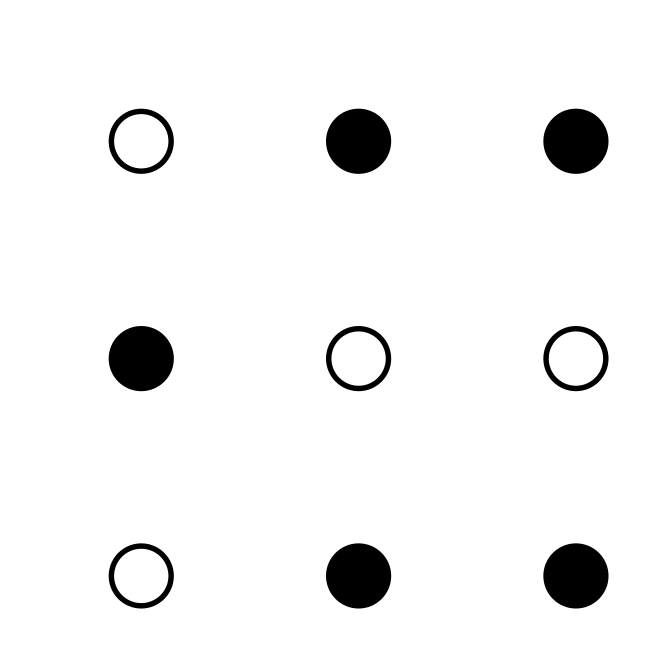
\includegraphics[width=0.3\textwidth]{images/kakeya_ex_f32.png}}
\caption{An example of a Kakeya set (shaded) in $\FF_3^2$.}
{\label{kak_ex_f32}
\end{figure}


\section{Introduction to Finite Fields}
\begin{definition}[Finite Field]
    A finite field, $\FF$, is a finite set that forms a field. That is, it is closed under addition, subtraction, multiplication, and non-zero division. 
    The number of elements of a finite field, $|\FF|$, is called the order of the finite field.
\end{definition}
A finite field of order $q$ exists if and only if $q = p^k$ for some prime $p$ and integer $k$. 

\begin{lemma}
    Each element $X$ in a finite field $\FF$ satisfies the identity:
    $$X^{|\FF|} - X =0$$
    identically in $\FF$.
    \label{lem:finite-fields-poly-identity}
\end{lemma}
This lemma follows immediately from Fermat's Little Theorem.
\todo{more needed here}




\section{Combinatorial attempts at the proof} \todo{this section sucks, rewrite!}
We fix a finite field $\FF = \FF_{p^k}$.
\subsection{Bush Argument}
Bourgain produced one of the first non-trivial estimates of the dimension in 1991.\cite{BUSH1991} We present the finite field analogue of his argument here.\cite{GUTH2016}
\begin{theorem}[Bush Argument]
If $l_1, \dots, l_M$ are lines in $\FF^n$, then the number of points in their union is at least 
$$\frac12 M^{1/2} |\FF|$$
In particular, if $A$ is a Kakeya set, then we have:
$$|A| \gtrsim |\FF|^{\frac{n+1}{2}}$$
\end{theorem}

\prf{Let $X$ be the union of the lines $l_1, \dots, l_M.$ Each of these lines contains $|\FF|$ points of $X$,
so we have $|\FF|M$ points to distribute over $X$. By the pigeonhole principle, there is a point $x \in X$ which lies in at least $|\FF|M |X|^{-1}$ of the lines $l_i$.
\todo{ Im not sure what to expand on here - we could contradict by saying if this wasn't the case but that seems verbose}

These set of lines $l_i$ through $x$ is called the bush of $x$. These lines are disjoint except at $x$, and their union 
lies in $X$. So we have:
\[
(|\FF| -1) |\FF| M |X|^{-1} \leq |X|.
\]
Rearranging we get:
\[
\frac12 |\FF| M^{1/2} \leq |X|    
\]
A Kakeya set $A \subset \FF^n$ contains at least $ |\FF|^{n-1}$ lines. Setting $M= |\FF|^{n-1}$ yields:
\[
\frac12 |\FF||\FF|^{\frac{n-1}{2}} \sim |\FF|^{\frac{n-1 +2}{2}} =  |\FF|^{\frac{n+1}{2}} \lesssim |A|.
\]
}


\subsection{Hair Brush Argument}
Due to Wolff. \cite{WOLFF1995}

\begin{theorem}[Hair Brush Argument]
    Suppose $l_1, \dots , l_M$ are lines in $\FF^n$, and that at most $|\FF| +1$ of the lines lie in any plane.
    Then their union has cardinality at least 
    \[
        \frac{1}{3}    |\FF|^{3/2} M^{1/2}.
    \]
    In particular, if $A$ is a Kakeya set, then we have:
    \[
        |A| \gtrsim |\FF|^{\frac{n+2}{2}}    
    \]
\end{theorem}
\begin{proof}
    Let $X = \cup_i l_i$. If $l_i$ is a line in $A$, then the hairbrush with stem $l_i$ is
    defined to be the set of lines $l_j$ which intersect $l_i$. An average point of $X$ lies in $|\FF|M |X|^{-1}$ lines $l_i$.
    If each point of X was about average, then each hairbrush would contain $\gtrsim |\FF|^2 M |X|^{-1}$ lines. We claim
    that there is always at least one hairbrush with $\geq (1/2)|\FF|^2M |X|^{-1}$ lines.  

   \todo{ Finish this proof}
\end{proof}

\section{Dvir's Proof}

In finite fields Kakeya's conjecture is as follows:
\thm{Kakeya Conjecture in Finite Fields}{If $A\subset \FP^n$ contains a translate of every line, then $|A| \gtrsim_n p^n $. \label{KakeyaConjecture}}

We shall prove this theorem via 3 surprisingly simple lemmas. This formulation of Dvir's proof is due to Gowers.\cite{GOW2020}

\begin{lemma}[Parameter Counting] 
Let $\KK$ be a (not necessarily finite) field. If $A \subset \KK^n$ and $|A| < {{n+D} \choose {n}}$, there exists a non-zero polynomial $P(x_1,\dots, x_n)$ of degree $D$ that vanishes on $A$. \label{paramcounting}
\end{lemma}

\prf{ We first show the dimension of $\text{Poly}_D (\KK^n)$ is ${D+n} \choose{n}$. A basis for $\text{Poly}_D (\KK^n)$ is given by monomials of the form $x_1^{D_1}\dots x_n^{D_n}$, where $\sum_i D_i \leq D$, hence we just need to count the number of monomials.

We can map a monomial $x_1^{D_1}\dots x_n^{D_n}$ to a string of $D$ $\star$'s and $n$ $|$'s as follows. Begin with $D_1$ $\star$'s, then place one $|$. We put now $D_2$ $\star$'s, and place a second $|$. We continue until we have placed $D_n$ $\star$'s followed by an $n^{\text{th}}$ $|$. Finally we place $D - \sum_i D_i \star$'s. This is a bijective map between the monomials in $\text{Poly}_D (\KK^n)$ and all the strings of $D$ $\star$'s and $n$ $|$'s. To count the strings, fix the $n$ $|$'s. Now we have $n+1$ bins to distribute our $D$ $\star$'s. 
Therefore we have by the stars and bars theorem:
$$\text{Poly}_D (\KK^n) = {{n+1 + D - 1} \choose{n+1 -1}} = {{n+D} \choose{n}}.$$

Let now $p_1, \dots, p_{|A|}$ be the points of $A$. We consider the evaluation map $E: \text{Poly}_D (\KK^n) \to \KK^{|A|}$ defined by:
$$E(Q) = \left(Q(p_1), \dots, Q(p_{|A|})\right).$$

This map is clearly linear. Its kernel $\ker E$ is exactly the set of polynomials in $\text{Poly}_D (\KK^n)$ that vanish on $A$. By assumption, the dimension of $\text{Poly}_D (\KK^n)$ is greater than $A$, so the dimension of the domain of $E$ is greater than the codomain of $E$. By the rank-nullity theorem, we conclude $E$ must have a non-trivial kernel. Thus there exists a non-zero polynomial $P \in \text{Poly}_D (\KK^n)$ that vanishes on $A$.} 


Note that if $D=|\FF|-1$, and $|A| \leq {{|\FF|+n-1} \choose{|\FF|-1}} = { {|\FF|+n-1} \choose{n}}$ we have a polynomial of degree $|\FF|-1$ that vanishes on $A$. Since $\frac{|\FF|^n}{n!} < {{|\FF|+n-1} \choose{n}}$,we can definitely find such a polynomial when $|A| \leq \frac{|\FF|^n}{n!}$.


\lem{Suppose $A \subset \FF^n$ contains a line in every direction, and suppose that there exists a non-zero polynomial $P$ with degree $D<|\FF|$ that vanishes on $A$. Then there exists a non-zero degree $D$ polynomial $\bar{P}$ that vanishes everywhere on $\FF^n$. \label{kaklem2}}

\prf{ Choose a line in $A$, say $\ell = \{x+tz : t\in \FF \}$ with $x\in \FF^n$ and $z \in \FF^n / \FF^{\times}$. Now we consider the restriction of our polynomial $P$ to the line $\ell$, $P_{|\ell}$ .
Recall $P$ is a sum of monomials, and we use multi-index notation here with $\alpha = (\alpha_1, \alpha_2, \dots, \alpha_n), \ \alpha_i \in \NN \cup \{0\}$ and $|\alpha| =  \sum \alpha_i$. $P$ can be written as:
$$P(x_1,x_2, \dots, x_n) = \sum_{|\alpha| \leq D} c_{\alpha} x_1^{\alpha_1}x_2^{\alpha_2}\dots x_n^{\alpha_n}. $$
Now $P_{|\ell}$ can be written:
$$P_{|\ell} = P(x+tz) = Q_{x,z}(t) = \sum_{|\alpha| \leq D} c_\alpha \prod_{i} (x_i + t z_i)^{\alpha_i}.$$
We now wish to examine the degree $D$ term of $Q$, which is achieved by picking the $tz_i$ terms from each bracket in the product above. This gives the degree $D$ component of $Q$, $Q_{x,z,D}$, which has the form:
$$Q_{x,z,D} = t^D Q_D(z) = t^D \sum_{|\alpha| = D} c_\alpha \prod_i z_i.$$

Now if $P_{|\ell}$ vanishes everywhere on $\ell$, since its dependence on $t$ is given by a polynomial of degree less than $|\FF|$, all its coefficients must be zero. 
This is clear from the factor theorem, as we could write the roots of $P_{|\ell}$ as $(t-k_1)(t-k_2)\dots(t-k_{|\FF|})$, but this contradicts the fact $P$ is of degree $D < |\FF|$.

Notice that $Q_{x,z,D}$ no longer depends on $x$, but on $z$ alone. In particular $Q_D(z) = 0$, but $z$ was an arbitrary element of $\FF^n / \FF^{\times}$, and $Q_D(z)$ also vanishes at zero, so it vanishes everywhere. Thus we can pick $\bar{P}$ = $Q_D$, and we are done.
}





\lem{Let $P$ be a non-zero polynomial on $\FF^n$ with degree less than $|\FF|$. Then $P$ does not vanish everywhere. \label{kaklem3}}

\prf{ We proceed by induction on $n$. For $n=1$, a non-zero polynomial that vanishes everywhere has $|\FF|$ roots, so must be at least of degree $|\FF|$.
Let us assume that the statement holds in $\FF^{n-1}$, we now prove it must also hold for $\FF^N$.

We let $x_1, \dots ,x_n$ be coordinates on $\FF^n$, and we write $P$ in the form:

$$P(x_1, \dots ,x_n) = \sum_{j=n}^{|\FF|-1} P_j(x_1, \dots x_{n-1}) x_n^j.$$

Each $P_j$ are polynomials in $x_1, \dots x_{n-1}$ of degree less than $|\FF|$. Fix $x_1, \dots x_{n-1}$, and let $x_n$ vary. Now we have a polynomial in $x_n$ of degree less than $|\FF|$ that vanishes for all $x_n \in \FF$. By the base case this must be the zero polynomial. So each $P_j(x_1, \dots, x_{n-1}) = 0$ for all $j$ and for all $(x_1, \dots x_{n-1}) \in \FF^{n-1}$. Now by induction on $n$, each $P_j$ is the zero polynomial. Then $P$ is the zero polynomial as well. 

}

\begin{proof} [Proof of Theorem \ref{KakeyaConjecture}] 
Assume $A \subset \FF^n$ is a Kakeya set, and that $|A| \leq \frac{|\FF|^n}{n!}$. Then by \ref{paramcounting} we can find a 
non-zero polynomial, say $P$, that vanishes on $A$. Now by \ref{kaklem2} there exists a non-zero polynomial $\bar{P}$ that vanishes everywhere on $\FF^n$, and has degree less than $|\FF|$.
Finally $\ref{kaklem3}$ says that such a $\bar{P}$ is necessarily the zero polynomial, a contradiction. We conclude that $|A| > \frac{|\FF|^n}{n!}$, or in other words:
$$
|A| \gtrsim_n |\FF|^n.
$$
\end{proof}